\documentclass[9pt]{beamer}
%\usetheme[background=light]{metropolis}
\usetheme{Copenhagen}
\usecolortheme{seagull}
%\setmonofont{Ubuntu Mono}

\usepackage[utf8]{inputenc}

\title{Macaroons}
\subtitle{Cookies with Contextual Caveats for Decentralized Authorization in the Cloud}
\author{Rihan Pereira, MSCS}
\institute[California State University, Channel Islands]
{
  %\inst{1}%
  COMP 524 - Security, Fall 2018\\
  Department of Computer Science\\
  California State University, Channel Islands
}
\date{\today}

% Delete this, if you do not want the table of contents to pop up at
% the beginning of each subsection:
%\AtBeginSubsection[]
%{
%  \begin{frame}<beamer>{Outline}
%    \tableofcontents[currentsection,currentsubsection]
%  \end{frame}
%}

\begin{document}

% title frame, marks the beginning of presentation
\begin{frame}[plain]
  \frametitle{}
  \titlepage
\end{frame}

% table of contents a.k.a outline
\begin{frame}[plain]
  \frametitle{Agenda}
  \tableofcontents
\end{frame}

% real meat of the presentation
% -------------------------------------

\section{Web Cookies}
\begin{frame}{Web Cookies}
  \begin{columns}
    \column{0.7\textwidth}
    \begin{itemize}
    \item solves user identity problem in dynamic web sites.
      \pause
    \item fundamentally used to store session IDs
      \pause
    \item still in use today!
    \end{itemize}

    \column{0.3\textwidth}
    
  \end{columns}
\end{frame}

% -------------------------------------
\begin{frame}
  \centering{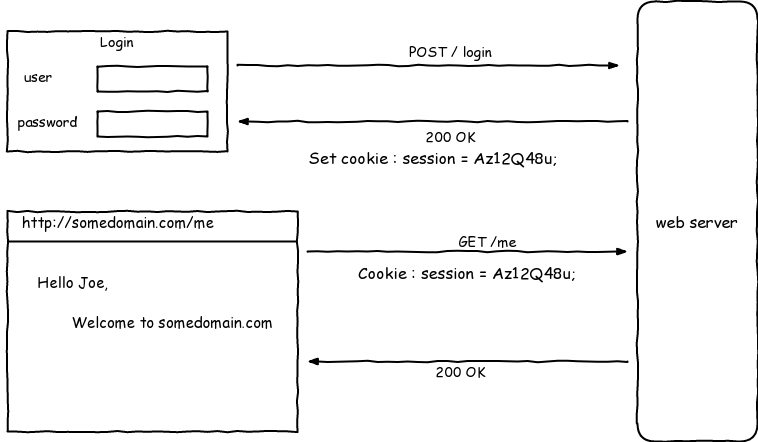
\includegraphics[width=100mm, height=60mm, scale=0.1]{img/web_cookies/webcookie_construct.png}}
\end{frame}

% -------------------------------------

\subsection{Vulnerabilities}
\begin{frame}{Vulnerabilities}
  \begin{itemize}
    \item Man in the middle attack
    \item Cross site resource fogery(CSRF)
  \end{itemize}
\end{frame}

% -------------------------------------

\subsection{CSRF attack}
\begin{frame}{CSRF attack}
  Executes unwanted actions on a dynamic site in which they are currently authenticated.
\end{frame}

% -------------------------------------

\begin{frame}{fix 1 - using a csrf token}
  \centering{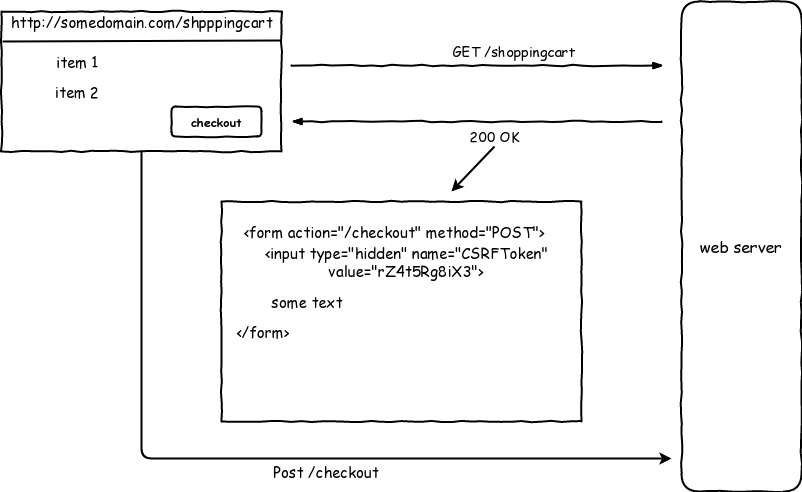
\includegraphics[width=100mm, height=60mm, scale=0.1]{img/web_cookies/csrf_token.png}}
\end{frame}

% -------------------------------------

\begin{frame}{fix 2 - double submit cookie}
  \centering{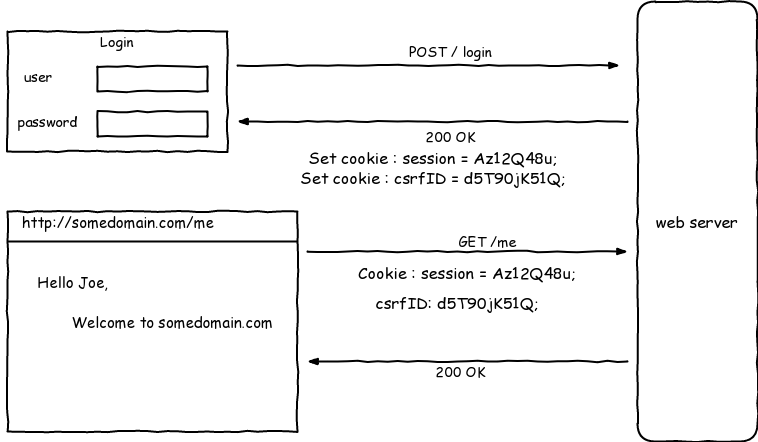
\includegraphics[width=100mm, height=60mm, scale=0.1]{img/web_cookies/double_submit_cookie.png}}
\end{frame}

% -------------------------------------

\subsection{session limitations}
\begin{frame}{session limitations}
  \begin{itemize}
  \item web cookies are opaque
    \pause
  \item dont solve access-control problem    
    \pause
  \item lookup server state on every request
    \pause
  \item really not good for distributed/clustered applications
  \end{itemize}
\end{frame}

% -------------------------------------

\section{Token Authentication}
\begin{frame}{Token Authentication}
  \begin{itemize}
    \item self-contained chunk of information
      \pause
    \item intrinsic value in that string
  \end{itemize}
\end{frame}

% -------------------------------------

\subsection{OAuth 2.0}
\begin{frame}{OAuth 2.0}
  \centering{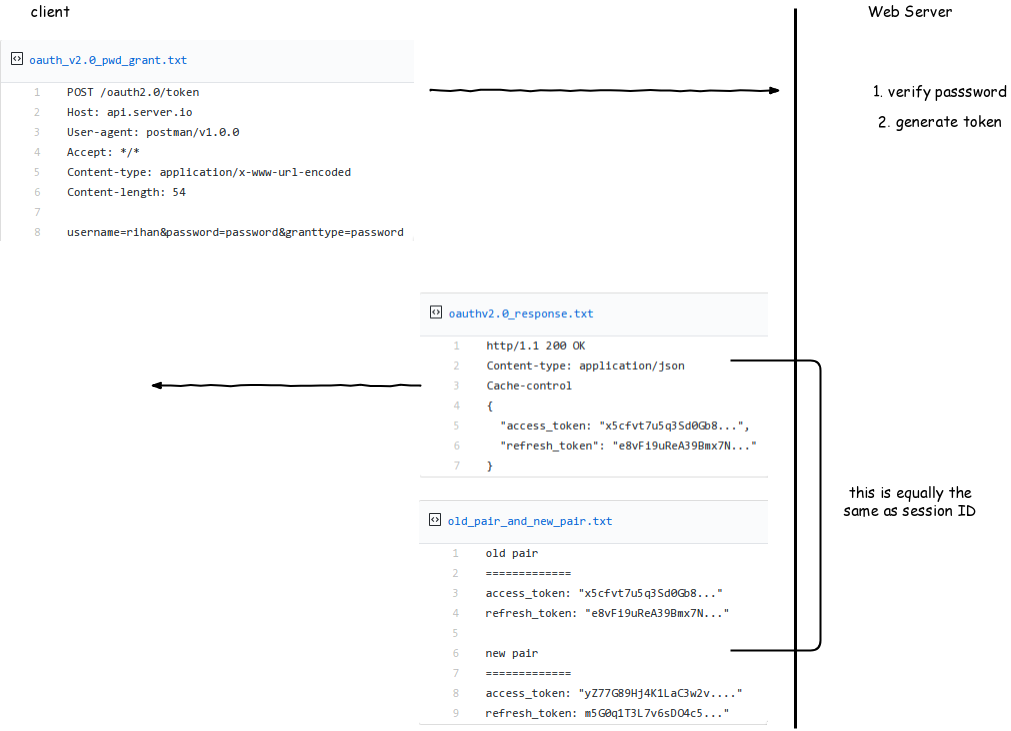
\includegraphics[width=100mm, height=60mm, scale=0.1]{img/token_auth/oauth_pwd_grant.png}}
  \pause
  using access token - Authorization Bearer "x5cfvt......"
\end{frame}

% -------------------------------------

\subsection{JSON Web Tokens(JWT)}
\begin{frame}{JSON Web Tokens(JWT)}
  \begin{columns}
    \column{0.7\textwidth}
    \centering{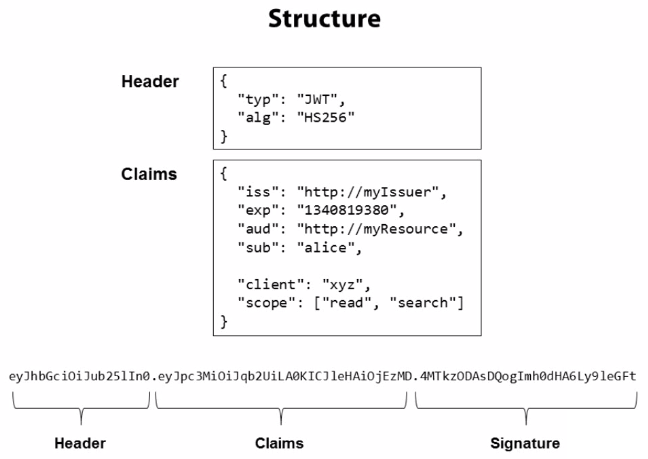
\includegraphics[width=70mm, height=50mm, scale=0.1]{img/token_auth/jwt.png}}
    \column{0.4\textwidth}
    \begin{itemize}
    \item URL-safe, self-contained string, digitally signed.
      \pause
     \item client aware access-control. 
    \end{itemize}
  \end{columns}
\end{frame}


\subsection{OAuth + JWT}
\begin{frame}{OAuth + JWT}
  \begin{columns}
    \column{0.7\textwidth}
    \centering{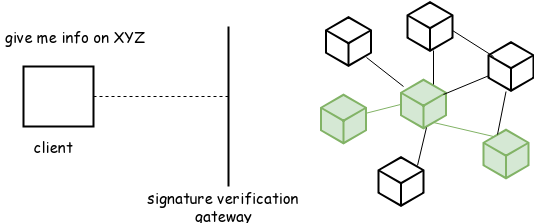
\includegraphics[width=70mm, height=40mm, scale=0.1]{img/token_auth/jwt_graph.png}}
    \column{0.4\textwidth}
    \begin{itemize}
    \item 3 tier access token
      \pause
    \item Instead of state on the server side, state is on the client side
      \pause
     \item reduced data access scope
    \end{itemize}
  \end{columns}
\end{frame}

% -------------------------------------

\subsection{OAuth + Signatures}
\begin{frame}{OAuth + Signatures}
  \begin{columns}
    \column{0.7\textwidth}
    \centering{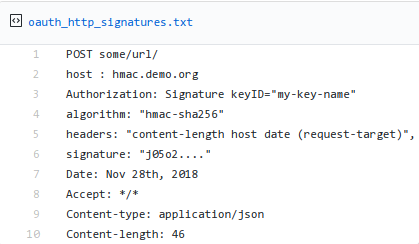
\includegraphics[width=70mm, height=40mm, scale=0.1]{img/token_auth/oauth_signatures.png}}
    \column{0.4\textwidth}
    \begin{itemize}
    \item no secret sent over the wire
      \pause
    \item symmetric key used between trusted entities
      \pause
    \item stateless
      \pause
    \item driving modern REST security these days.
    \end{itemize}
  \end{columns}
\end{frame}

% -------------------------------------

\section{Macaroons}
\begin{frame}
\end{frame}

\section{References}
\begin{frame}
  \bibliographystyle{unsrt}
  \begin{thebibliography}{99}
  \bibitem[Paper 1]{ref1} Arnar Birgisson, Joe Gibbs Politz, Ulfar Erlingsson, Ankur Taly, Michael Vrable, and Mark Lentczner,  \newblock \emph{Macaroons: Cookies with Contextual Caveats for Decentralized Applications in the Cloud}, \textbf{2015}.
  \bibitem[Paper 2]{ref2} \href{https://www.owasp.org}{https://www.owasp.org}
  \bibitem[Paper 3]{ref3} \href{https://jwt.io/}{https://jwt.io/}
  \bibitem[Paper 4]{ref3} \href{http://aosabook.org}{http://aosabook.org}
  \bibitem[Paper 5]{ref3} \href{https://oauth.net/2/}{https://oauth.net/2/}
  \end{thebibliography}
\end{frame}

\section{}
\begin{frame}{}
  \centering{Thank you! Questions ?}
\end{frame}
\end{document}
%%% Local Variables:
%%% mode: latex
%%% TeX-master: t
%%% End:
